\section{Paginazione}
La paginazione risolve il problema posto dalla frammentazione esterna consentendo la non contiguità degli indirizzi fisici, mantenendo invece la contiguità negli indirizzi logici.

\subsection{Implementazione}
Si divide la memoria fisica in blocchi di dimensione fissa, detti frame o pagine fisiche. Allo stesso modo si divide anche la memoria logica in blocchi della stessa dimensione.

La \textbf{tabella delle pagine}, tiene traccia delle relazioni tra memoria fisica e logica e tiene traccia delle pagine libere.

\spacer
Gli indirizzo logici generati dalla CPU vengono suddivisi in:
\begin{sitemize}
    \item \textbf{Numero di pagina:} indice che verrà usato nella tabella delle pagine.
    \item \textbf{Offset nella pagina:} definisce l'offset a partire dall'inizio della pagina
\end{sitemize}

\begin{figure}[H]
    \centering
    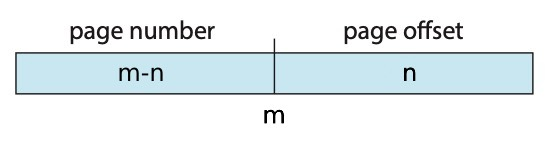
\includegraphics[width=0.35\linewidth]{assets/page-number-offset.jpg}
\end{figure}

Se lo spazio logico ha dimensione $2^m$ allora si hanno $2^{m-n}$ pagine di dimensione $2^n$. La scelta di m ed n detta anche la dimensione della tabella delle pagine.

\begin{figure}[H]
    \centering
    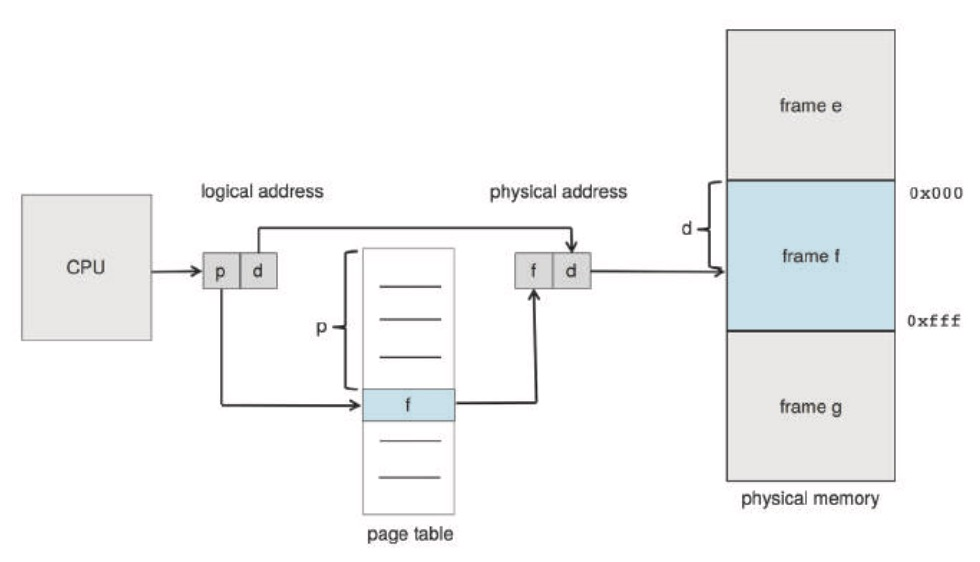
\includegraphics[width=0.48\linewidth]{assets/paginazione.jpg}
\end{figure}

\subsubsection*{Frammentazione}
Si ottiene della frammentazione interna quando un processo non occupa completamente un frame, ad esempio un processo di 72766 byte occupa 36 pagine da 2048 byte, ma l'ultima pagina viene riempita circa a metà.

\subsubsection*{Dimensioni dei frame}
Un'importante considerazione che deve essere fatta nell'architettura dell'elaboratore è la dimensione delle pagine.

Pagine più piccole permettono una minore frammentazione in quanto si possono meglio adattare alle dimensioni del programma, esse migliorano inoltre il principio di località.

Al contrario pagine più grandi riducono le dimensioni della page table e riducono il numero di page fault incontrati.

La soluzione adottata da molti sistemi operativi è quella di costruire pagine di diverse dimensioni così da potersi adattare ad ogni processo.

\subsubsection*{Pagine Bloccate}
In alcuni casi occorre mantenere delle pagine perennemente in memoria, come nel caso di operazioni di I/O tramite DMA, per questo motivo è possibile segnalare al pager delle pagine bloccate (\textit{pinned}) che non possono essere selezionate come vittime dall'algoritmo di sostituzione.

\subsection{Supporto Hardware}
Si utilizza una tabella delle pagine per ogni processo, essa risiede nella memoria principale e il processo ha un puntatore ad essa (PTBR) ed alla sua lunghezza (PTLR).

\spacer
Uno degli svantaggi di inserire la tabella delle pagine nella memoria principale è l'\textbf{aumento del tempo di accesso dati}, infatti per ogni richiesta devono essere fatte due richieste alla memoria, una alla tabella ad una all'indirizzo fisico.

\spacer
Una soluzione è il \textit{translation look-aside buffer (TLB)} che permette la ricerca in parallelo su una piccola tabella (64-1024 elementi). Essa può essere utilizzata come cache per la tabella delle pagine.

La TLB è più efficiente e sicura quando non viene condivisa tra più processi, ad ogni \textit{context switch} andrebbe fatto un \textit{flush} della memoria.
È possibile aggiungere un valore \textit{Address Space IDentifier (ASID)} che identifica il processo a cui appartiene l'associazione, questo permette di mantenere la TLB di un processo anche in un context switch.

\begin{figure}[H]
    \centering
    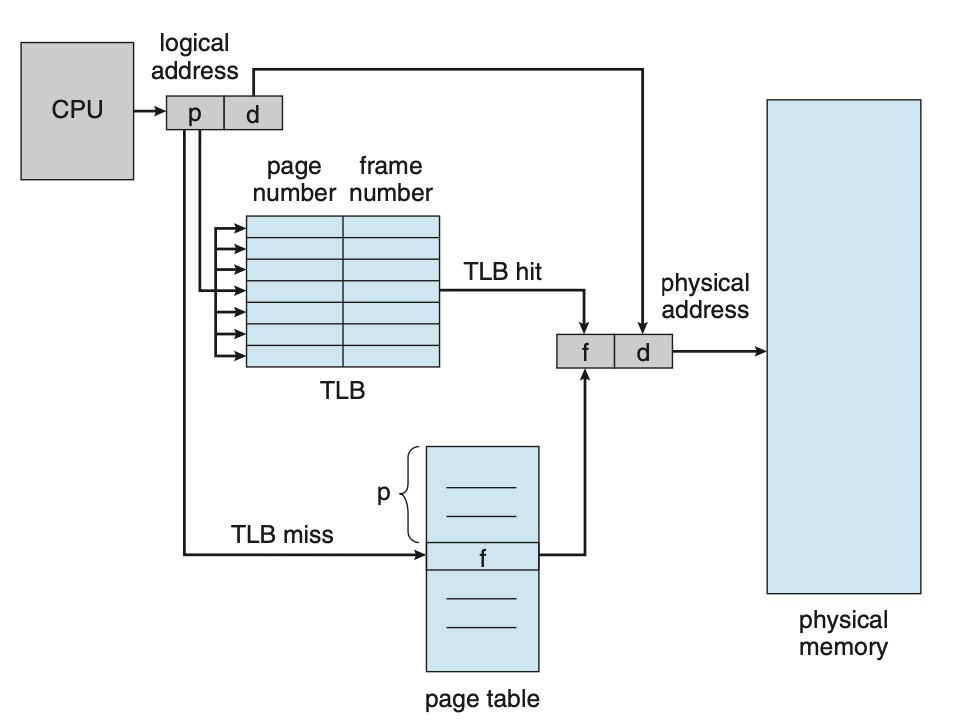
\includegraphics[width=0.5\linewidth]{assets/paginazione-tlb.jpg}
\end{figure}

\subsubsection{Page Fault}
Se un processo fa riferimento ad una pagina che al momento non è in memoria principale viene generato un \textbf{interrupt} di tipo page fault.

Il processo viene quindi sospeso finché il sistema operativo non carica la pagina mancante in memoria principale. Se la memoria è piena è necessario utilizzare un algoritmo di camnio pagina per scegliere quale pagina rimuovere.

\subsubsection{Protezione della Memoria}
Viene implementata grazie ad uno o più \textbf{bit di protezione} che determinano se una è possibile accedere una determinata pagina in lettura oppure lettura/scrittura.

\spacer
Inoltre viene aggiunto un \textbf{bit di validità}, esso permette di individuare le pagine che non appartengono agli indirizzi \textit{logici} del processo, questo viene poi segnalato all'utente tramite un'interrupt.

\subsection{Dimensioni della Tabella}
La tabella delle pagine può arrivare facilmente a dimensioni importanti, soprattutto quando se ne crea una per ogni processo, una rappresentazione naturale, ma inefficiente.

\subsubsection*{Tabella delle Pagine Invertita}
Una soluzione è costruire una tabella delle pagine invertita, la quale ha un elemento per ogni frame fisico e salva il frame logico e un identificatore del processo.


Questo riduce lo spazio totale usato dalle tabelle delle pagine ma incrementa il tempo di ricerca nella tabella.
Inoltre rende difficile la condivisione delle pagine fisiche tra processi.

\begin{figure}[H]
    \centering
    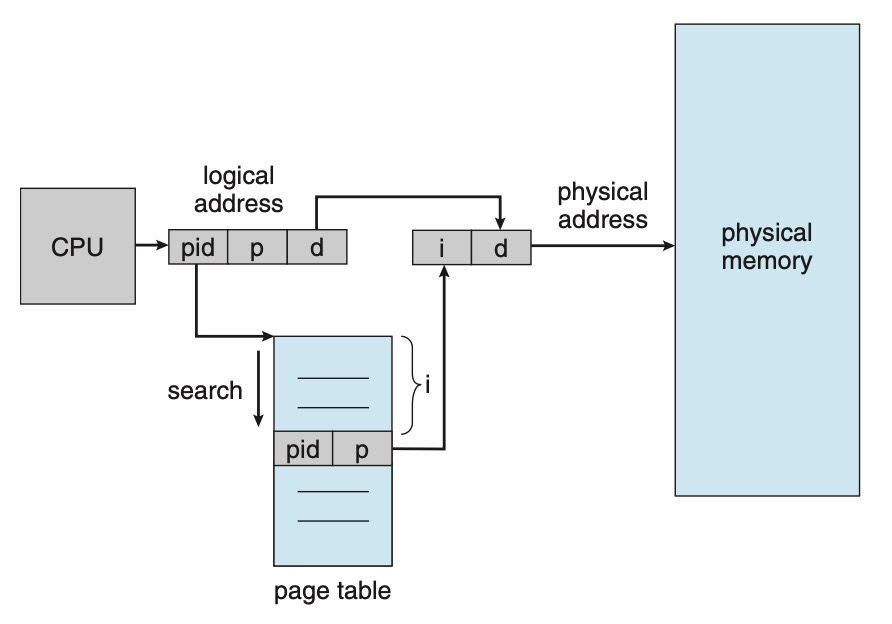
\includegraphics[width=0.45\linewidth]{assets/tabella-pagine-invertita.jpg}
\end{figure}

\subsubsection*{Paginazione Gerarchica}
L'idea con questa soluzione è quello di dividere lo spazio degli indirizzi logici in più tabelle delle pagine. Il caso più semplice è quello ottenuto utilizzando una paginazione a due livelli.

\begin{figure}[H]
    \centering
    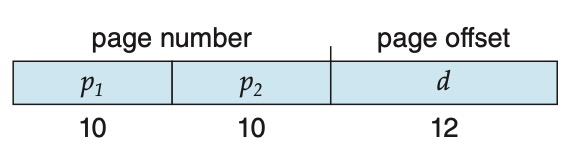
\includegraphics[width=0.35\linewidth]{assets/paginazione-doppia.jpg}
\end{figure}

$p_1$ viene utilizzato per indicizzare la tabella delle tabelle, mentre $p_2$ per indicizzare la tabella delle pagine.

\begin{figure}[H]
    \centering
    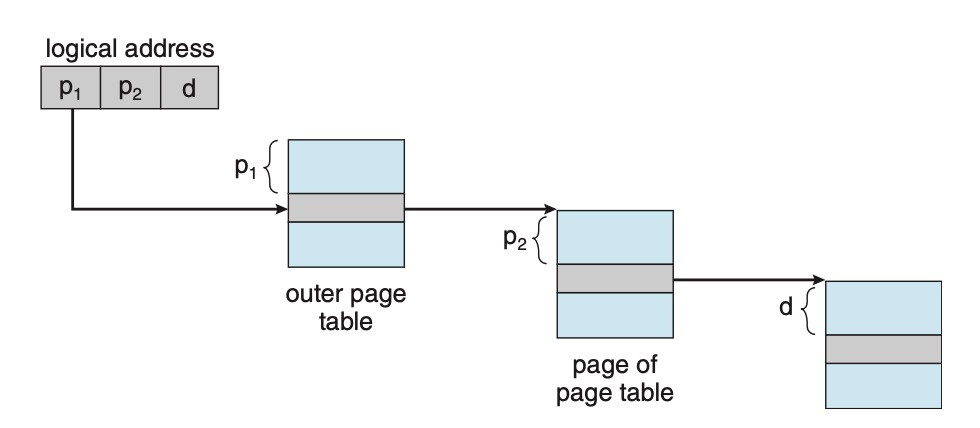
\includegraphics[width=0.5\linewidth]{assets/paginazione-gerarchica.jpg}
\end{figure}

Per le architetture a 64 bit questo tipo di paginazione necessita di troppi livelli di paginazione, è quindi da considerarsi inadeguata.

\subsubsection*{Tabella delle Pagine Hash}
Comunemente utilizzato per architetture a 64 bit.

L'elemento che viene inserito nella funzione di hash è il numero della pagina virtuale. Gli elementi della tabella sono liste concatenate, questo per gestire le eventuali collisioni dovute alla funzione di hash.

\spacer

In particolare ciascun elemento della tabella è composto da:
\begin{sitemize}
    \item Numero della pagina virtuale
    \item Numero della pagina fisica
    \item Puntatore al frame successivo
\end{sitemize}

\begin{figure}[H]
    \centering
    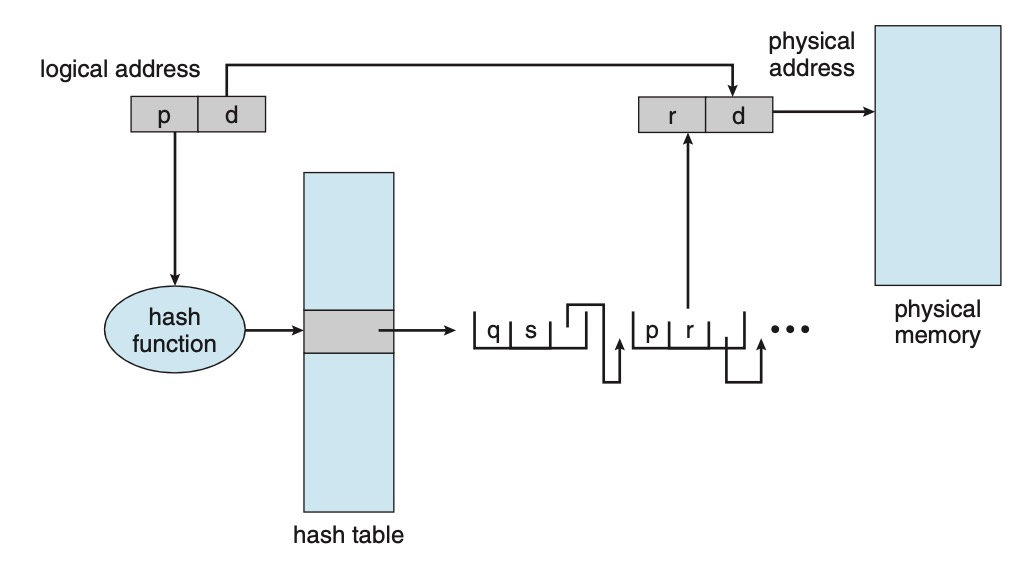
\includegraphics[width=0.5\linewidth]{assets/hashed-page-table.jpg}
\end{figure}

\begin{note}
    Per gli spazi a 64 bit si utilizza una tabella delle pagine a gruppi, ovvero una tabella hash dove ogni elemento contiene riferimenti alle pagine fisiche corrispondenti ad un gruppo di pagine virtuali contigue.
\end{note}

\subsubsection*{Segmentazione}
Gestisce la memoria in segmenti di dimensione variabile, questo è più vicino a come l'utente immagina l'organizzazione della memoria. Ogni segmento è un'unità logica:
\begin{sitemize}
    \item Procedure e funzioni
    \item Variabili
    \item Oggetti
\end{sitemize}

Si ha quindi una \textbf{tabella dei segmenti} per ogni processo che mappa gli indirizzi logici in coppie base, limite.

\begin{figure}[H]
    \centering
    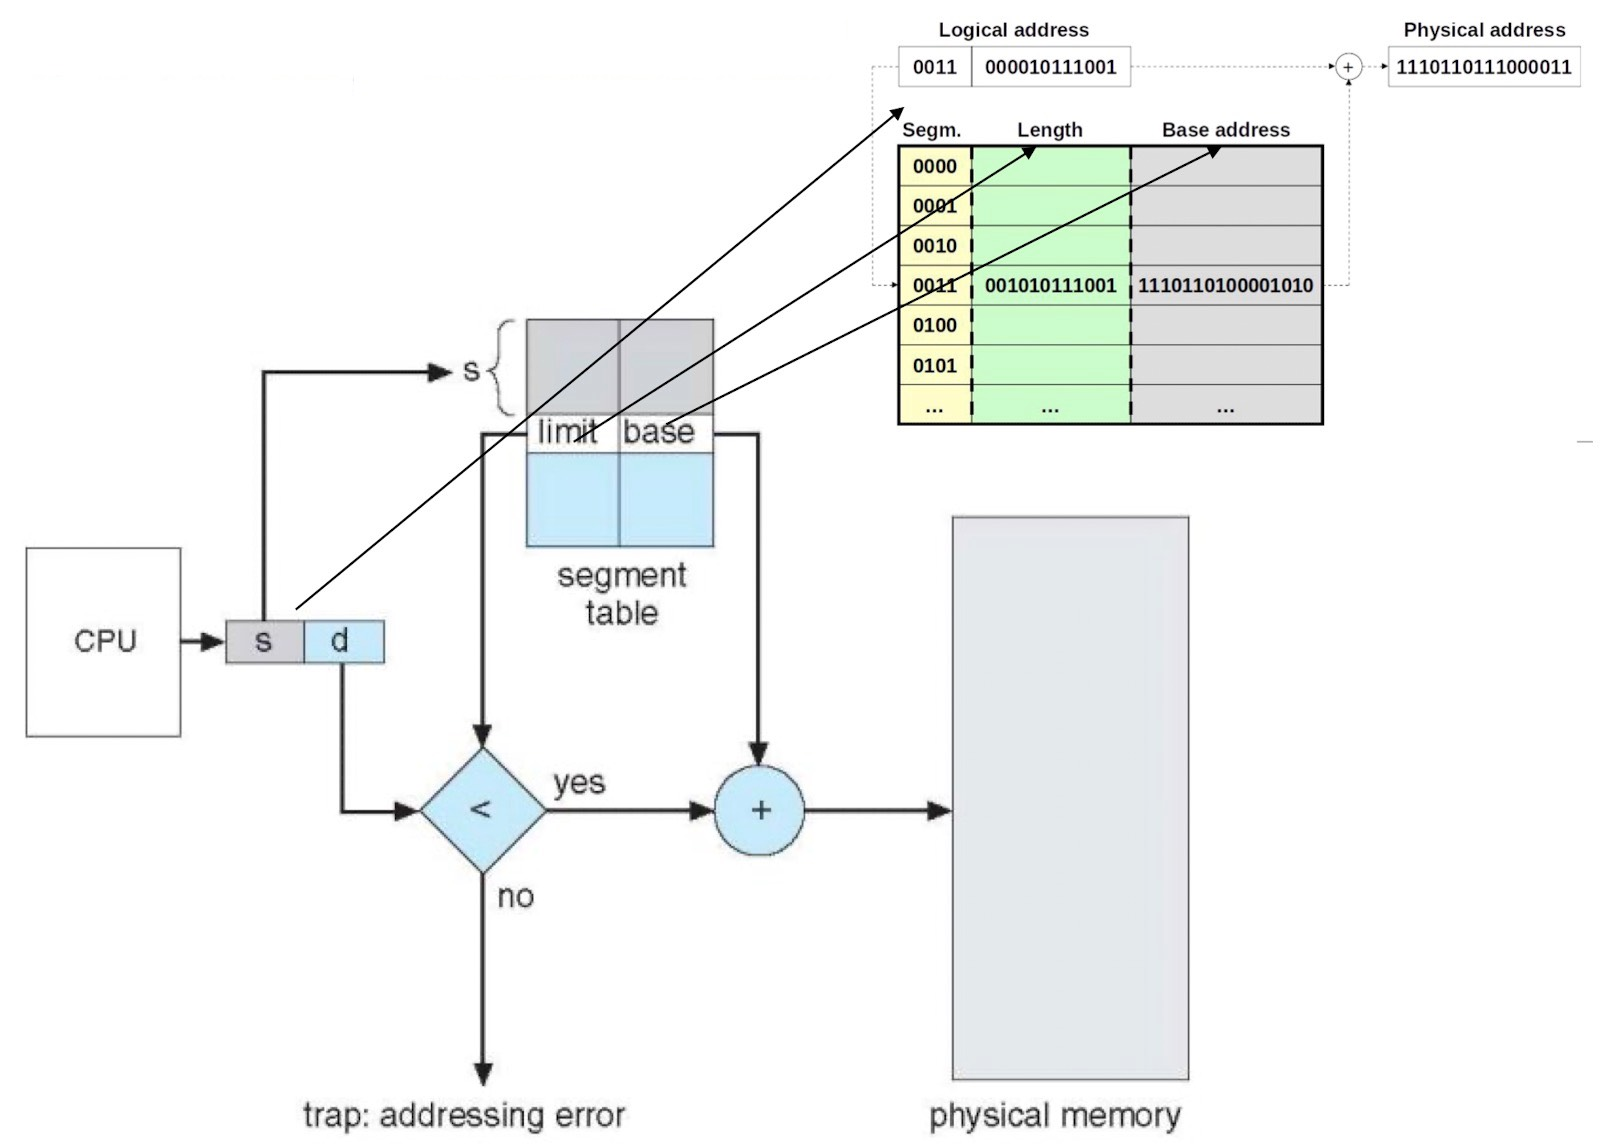
\includegraphics[width=0.48\linewidth]{assets/segmentazione.jpg}
\end{figure}

Due registri sono di particolare importanza in questo caso: STRB (\textit{Segment Table Base Register}) e STLR (\textit{Segment Table Length Register}).

\subsection{Implementazioni}
\subsubsection{Intel 32}
Il pentium supporta sia la segmentazione pura che la segmentazione mista a paginazione.

\begin{figure}[H]
    \centering
    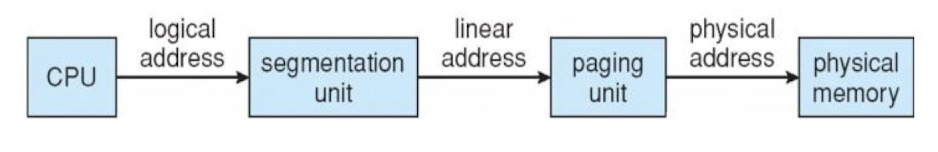
\includegraphics[width=0.5\linewidth]{assets/architettura-memoria-pentium.jpg}
\end{figure}

I segmenti possono essere di dimensione variabile, fino a 64 Kbyte, e possono essere al massimo $16 K$ per processo, di questi al massimo $8 K$ possono essere privati (Informazioni nella \textit{Local Descriptor Table, LDT}) e altri $8 K$ condivisi (Informazioni nella \textit{Global Descriptor Table, GDT}).

Il selettore è di 16 bit, dove 13 bit rappresentano l'indice del segmento ($2^{13} = 8192$), 1 bit per indicare LDT o GDT e 2 bit di protezione.
Altri 16 bit sono di offset.

\begin{figure}[H]
    \centering
    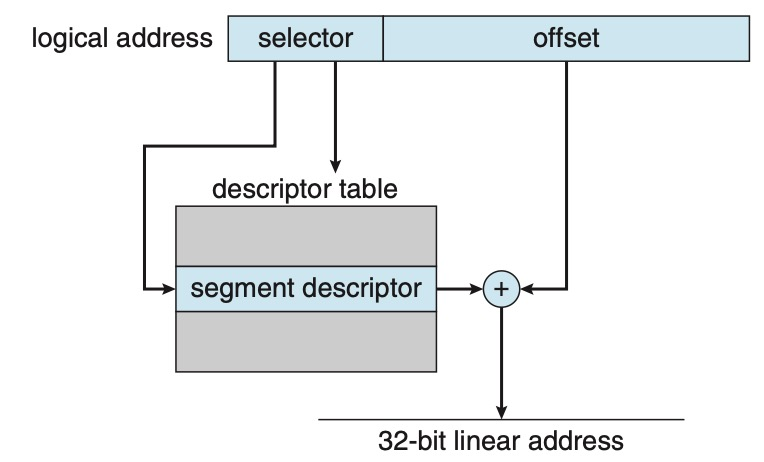
\includegraphics[width=0.5\linewidth]{assets/pentium-segmentation.jpg}
\end{figure}

Nella tabella vengono salvate anche altre informazioni, come un bit per indicare se il segmento è in memoria principale e uno per indicare se è stato modificato.

L'indirizzo ottenuto dalla segmentazione può essere paginato. Le pagine per il pentium possono essere di 4MB (1 livello) o 4KB (2 livelli) e viene usata una paginazione a due livelli.

\begin{figure}[H]
    \centering
    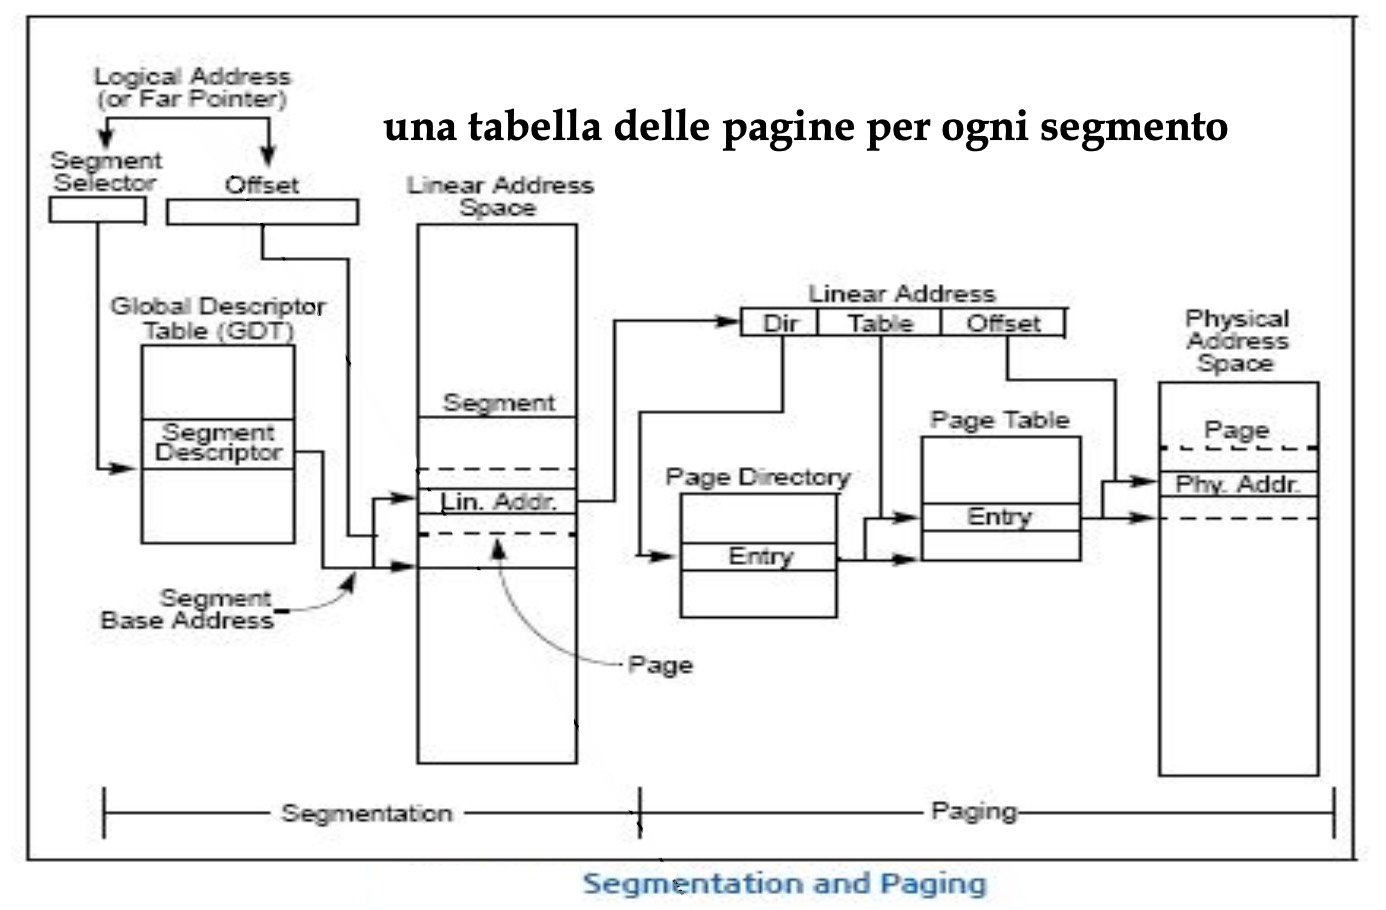
\includegraphics[width=0.5\linewidth]{assets/intel32-3.jpg}
\end{figure}

La dimensione della descriptor table viene aumentata nel tempo, prima a 24 e poi a 32 bit

\subsubsection{PAE}
Anche detto \textbf{Page Address Extension}, permette di raggiungere i 64 Gbyte di memoria.

Le principali modifiche all'architettura sono due: Viene inserito un ulteriore livello di paginazione, una page directory pointer table di 4 elementi e gli elementi della descriptor table arrivano a 64 bit, di cui solo 36 vengono utilizzati, arrivando così ad indicizzare 64 Gbyte di memoria.

\spacer
Le singole applicazioni possono, in generale, accedere solamente a 4GB di memoria, ma esse possono essere inserite in 64 Gbyte di memoria.

Inoltre è possibile per le applicazioni utilizzare delle system call per spostare il proprio spazio di indicizzazione, permettendo così di accedere ad una maggiore quantità di memoria RAM.

\begin{figure}[H]
    \centering
    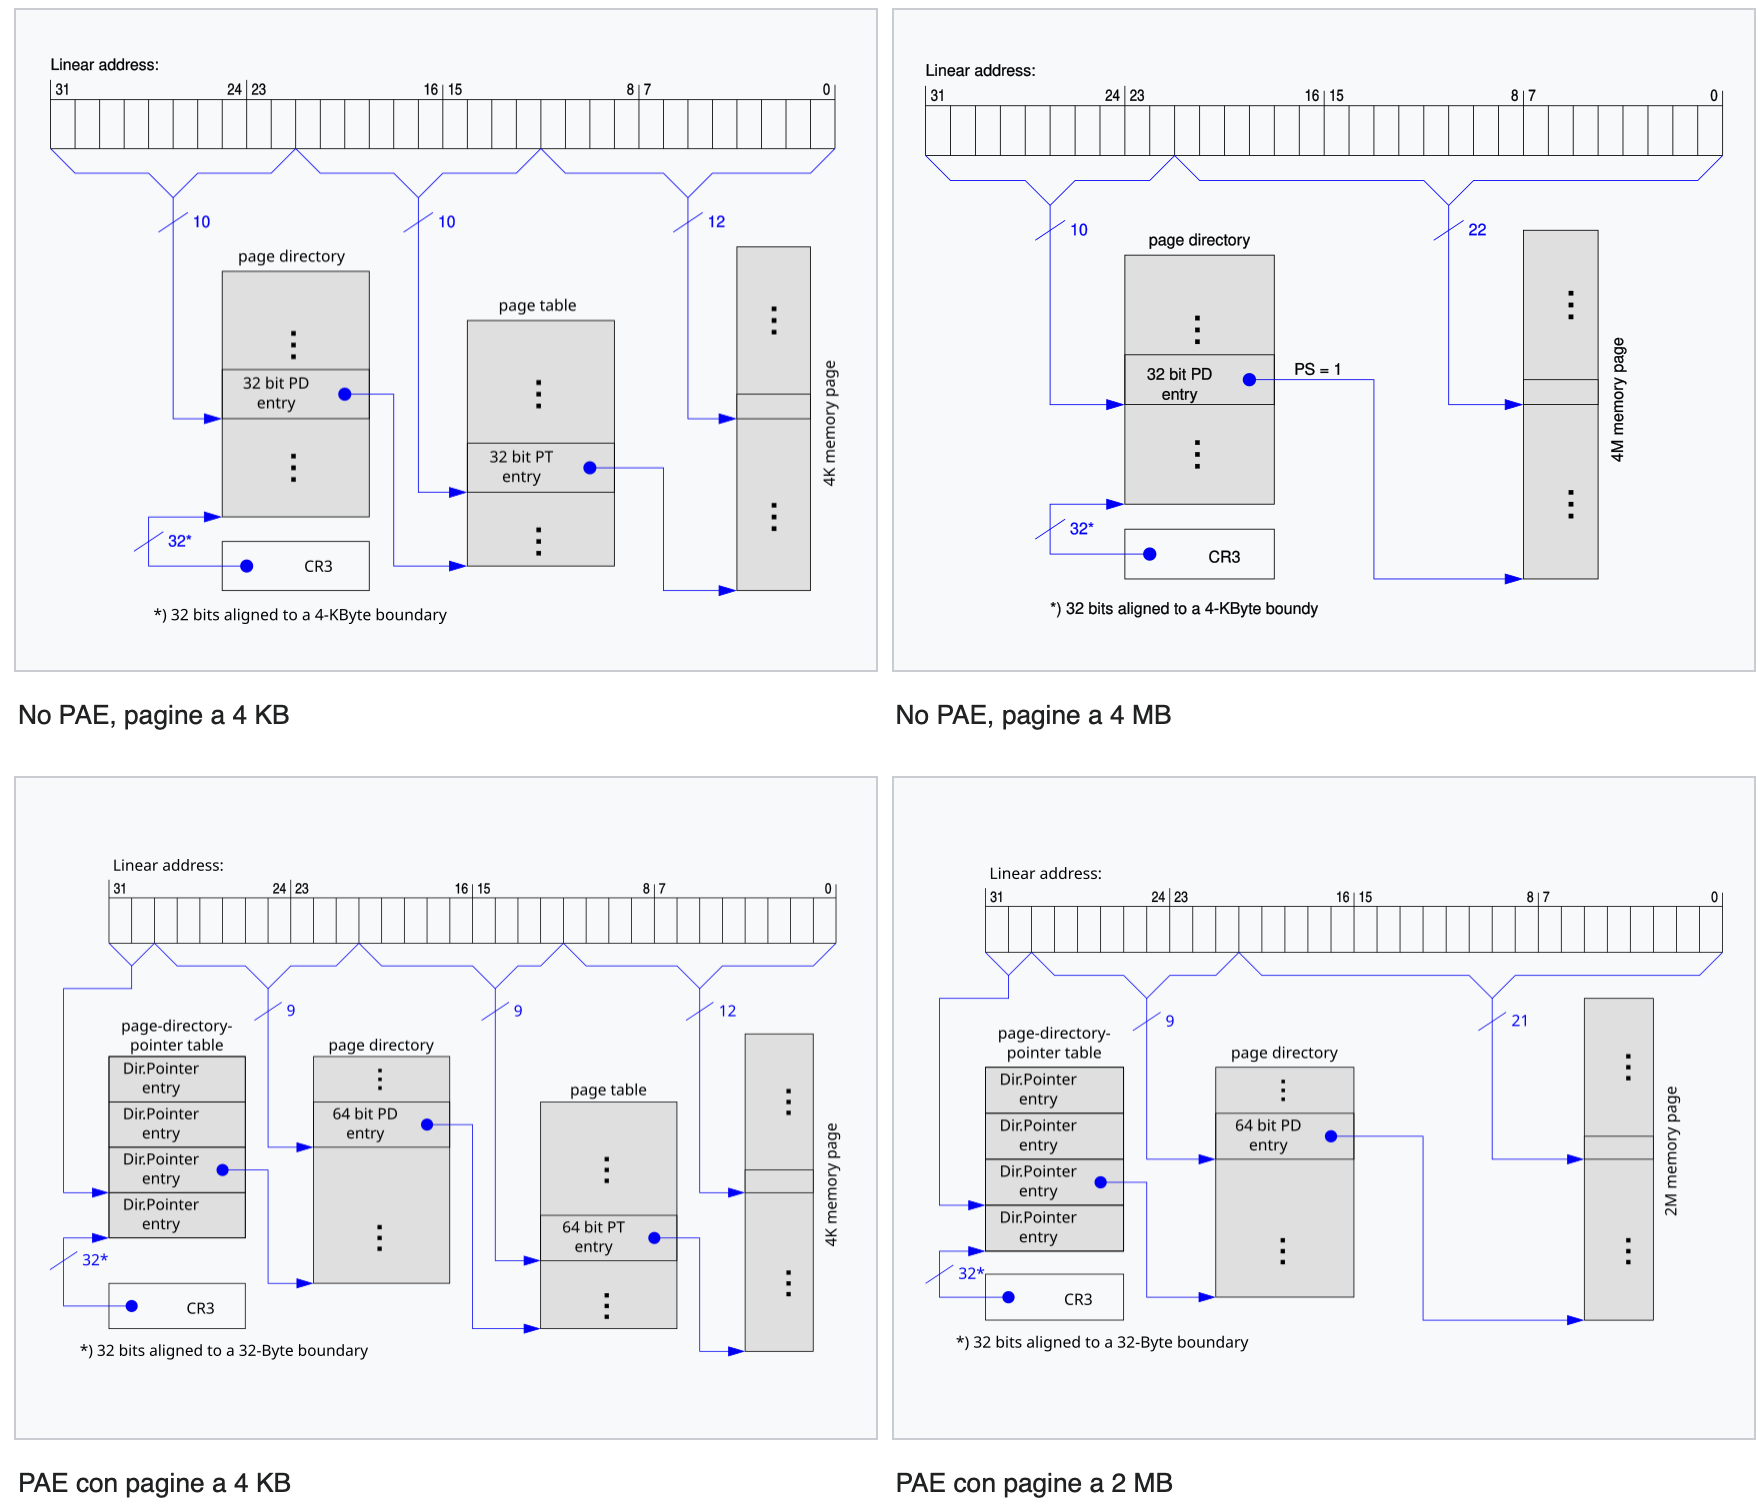
\includegraphics[width=0.75\linewidth]{assets/pae.png}
\end{figure}

\subsubsection{Intel x86-64}
Nei sistemi a 64 bit in realtà non se ne usano così tanti ($2^{64} = 17,179,869,184$ GB), gli indici sono tutti a 48 bit, lasciando inutilizzati i primi 16 bit.

L'architettura supporta pagine da 4KB, 2MB, 1GB.

\begin{figure}[H]
    \centering
    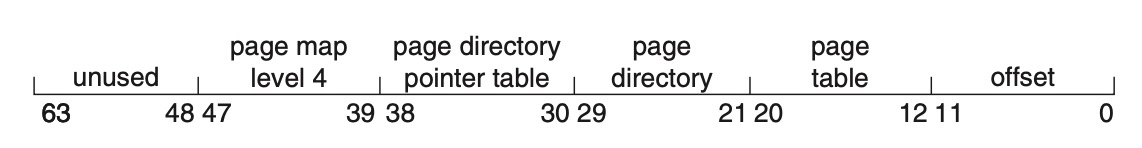
\includegraphics[width=0.6\linewidth]{assets/x64-address.jpg}
\end{figure}

È possibile utilizzare la PAE anche qui con l'obiettivo di portare gli indirizzi fisici da 48 a 52 bit.

\subsubsection{ARMv8}
Anche i processori ARM lavorano su 64 bit ed anche loro utilizzano fino a 4 livelli di paging ottenendo così pagine da 4KB, 2MB, 1GB.

\begin{figure}[H]
    \centering
    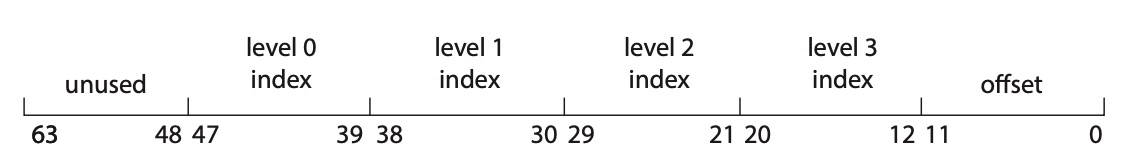
\includegraphics[width=0.6\linewidth]{assets/arm-address.jpg}
\end{figure}
